%!TEX root = ../master.tex
\chapter{Additional Kubernetes Concepts}
\label{appendix:kubernetes}
This appendix describes how a declarative definition of a production environment can be specified using YAML files. Furthermore, canary deployments, scaling, and databases in Kubernetes are described.


\section*{Declarative YAML Files}
Kubernetes promotes the use declarative definition of production environments. These definitions are often stored as YAML files. Listing~\ref{lst:cat_v1_deployment} shows a definition of a deployment of the cat-service from the demo project described Chapter~\ref{chap:tangible_cluster}. The definition specifies the deployment's labels and names. Furthermore, a replica set is defined in the \textit{spec} section. The replication set is specified to keep three replicas running of pods defined from the \textit{template}. Each pod contains a single container constructed from a specified Docker \textit{image}. The \textit{labels} on under the \textit{template} and \textit{metadata} plays an important role in regards to services.

\lstinputlisting[label={lst:cat_v1_deployment}, caption={Cat-service v1 deployment}]{scripts/cat-service-v1-deployment.yaml}

\noindent
The definition is saved as a YAML file and used by the command-line tool. The deployment of cat-service v1 could e.g. be created in the following way: \\

\newpage
\begin{lstlisting}
kubectl create -f cat-service-v1-deployment.yaml
\end{lstlisting}

\noindent
Listing~\ref{lst:cat_svc} shows a definition of a service. The important part is the \textit{selector} that decides which pods to route traffic to. The cat-service service filters pods by their labels. The cat-service service routes traffic to pods having the labels: \textit{app: cat-service} and \textit{tier:backend}. The previous deployment (Listing~\ref{lst:cat_v1_deployment}) contains these labels, and traffic will, therefore, be directed to the deployment's pods. Labels can be added and removed dynamically which leads to a loose and dynamic coupling between services and pods. Services stored in YAML files are also created using the command-line tool.

\lstinputlisting[label={lst:cat_svc}, caption={Cat-service service}]{scripts/cat-service-svc.yaml}


\section*{Canary Deployments}

One of the benefits of the loose coupling between services and pods is the ability to make canary deployments and the possibility of doing A\/B testing. A part of the incoming requests are routed to a new version while the majority of the requests will be directed to an old version. An example of this, and how it can be done using labels, is shown in Figure~\ref{fig:canary_deployment}.
\newpage
\begin{figure}[H]
    \centering
    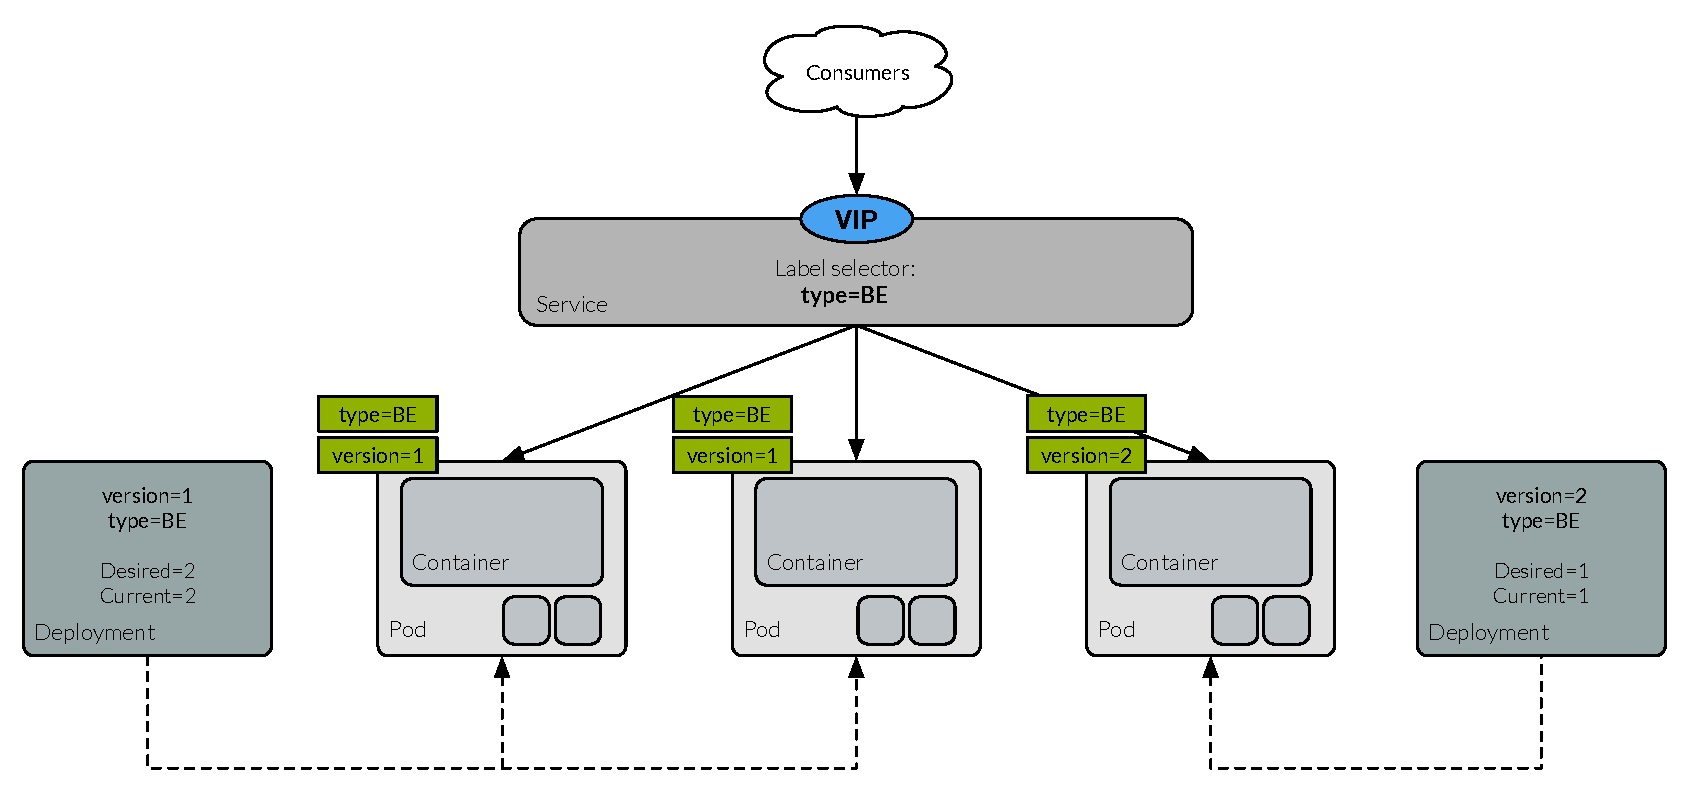
\includegraphics[width=15cm]{figures/kubernetes/canary_deployment}
    \caption{Canary Deployment}
    \label{fig:canary_deployment}
\end{figure}

\noindent The canary deployment is done using labels and two deployments. As it is seen in Figure~\ref{fig:canary_deployment} the service has a label selector \textit{type=BE}. There are two different deployments, one controlling version 1 of the application and one controlling and maintaining the desired state of version 2. Because both of the deployments' pods have the label \textit{type=BE} traffic is directed to them. Listing~\ref{lst:cat_v2_canary} shows the canary deployment containing version 2 of the cat-service. Notice that the \textit{app} and \textit{tier} labels are as the service expects, and that the image ends with the tag \textit{:v2}. \\


\lstinputlisting[label={lst:cat_v2_canary}, caption={Cat-service v2 canary deployment}]{scripts/cat-service-v2-canary.yaml}


\section*{Scaling}

Kubernetes features manual scaling and autoscaling. A deployment can easily be scaled by using the \textit{kubectl} command-line tool. The example below scales the number of running replicas to 10 for a deployment called NAME. \\

\begin{lstlisting}
kubectl scale deployment NAME --replicas=10
\end{lstlisting}

\noindent
Scaling replicas can also be achieved using YAML definitions. Instead of using the \textit{kubectl create} the  \textit{kubectl apply} command is used. \\


% AUTO
\noindent Kubernetes has an autoscaling mechanism is called \textit{Horizontal Pod Autoscaler (HPA)}. HPA allows to automatic scaling of the number of pods in a replica set or a deployment based on observed CPU utilization. This mechanism is implemented as a Kubernetes API resource and a controller. The resource describes the behavior of the controller, whereas the controller periodically adjusts the number of replicas to match the average CPU utilization to the target specified by the user. An example of this can be seen in Figure~\ref{fig:hpa}. 

\begin{figure}[H]
    \centering
    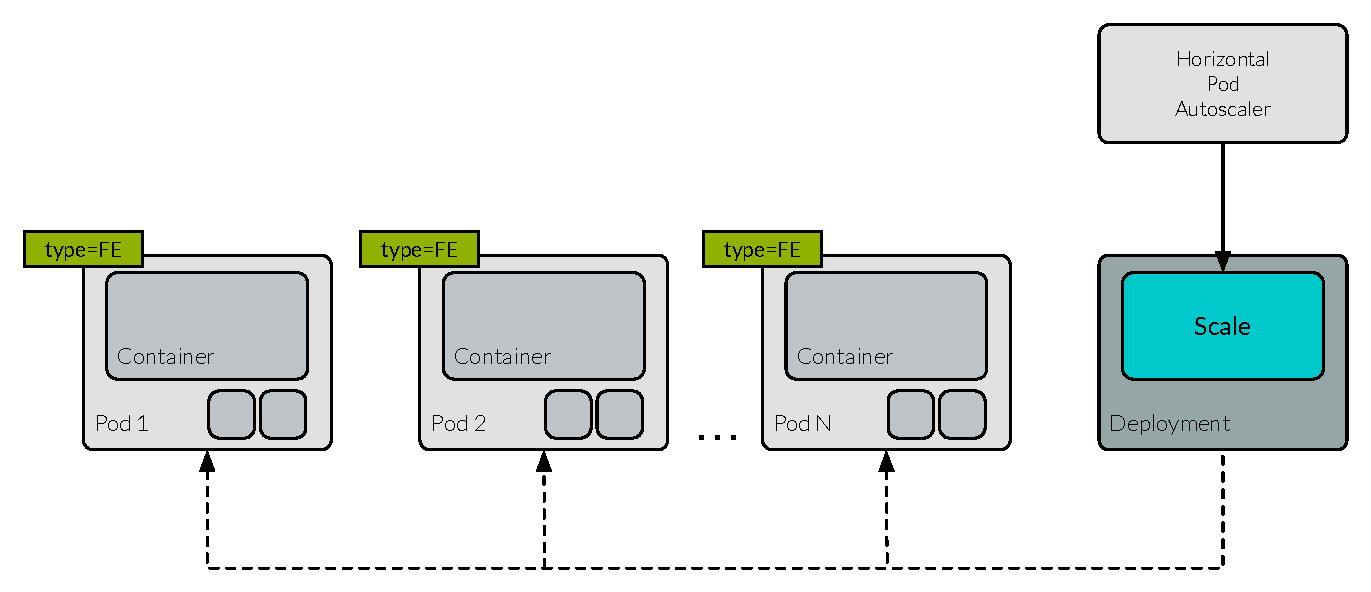
\includegraphics[width=15cm]{figures/kubernetes/autoscale}
    \caption{Horizontal Pod Autoscaler}
    \label{fig:hpa}
\end{figure}


\section*{Databases in a Dynamic Environment}
The role of databases has not been the focus of this master's thesis, but because it is an important part of applications the options in Kubernetes will be described in this section. Databases in dynamic and stateless environments such a Kubernetes is a challenge. Packaging a database in a Kubernetes pod and saving data in a container is not a stable solution because pods are ephemeral instead of long-lasting and durable. Three available database solutions described by Dorsey\footnote{\url{https://www.youtube.com/watch?v=DGlQgNmobuc}} are described in this section: outside of the cluster, adapting to the cluster, and cluster native.


\subsection*{Outside of the Cluster}
The first approach is to keep the database out of the cluster and have applications connect to a database outside the Kubernetes cluster. The database can be an already running database. Moving the data away might, though, lead to higher latencies depending on the database's location.

\begin{figure}
    \centering
    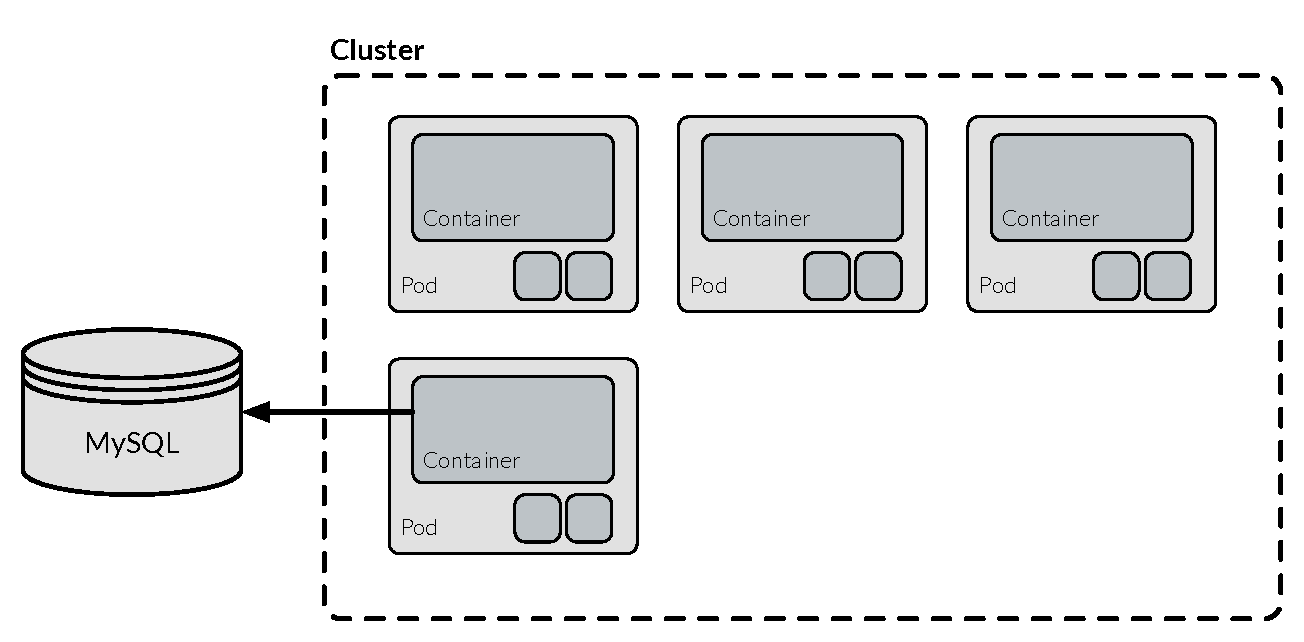
\includegraphics[width=12cm]{figures/appendix/database_outside_cluster}
    \caption{Database outside Cluster}
    \label{fig:db_outside_cluster}
\end{figure}


\subsection*{Adapt to the Cluster}
In Kubernetes, volumes can be mounted in pods. Thereby databases can be started in containers without storing data in an ephemeral container but instead stored on the external volume. The volume can e.g. be a networked file share (NFS) or storage from a cloud provider.

\begin{figure}
    \centering
    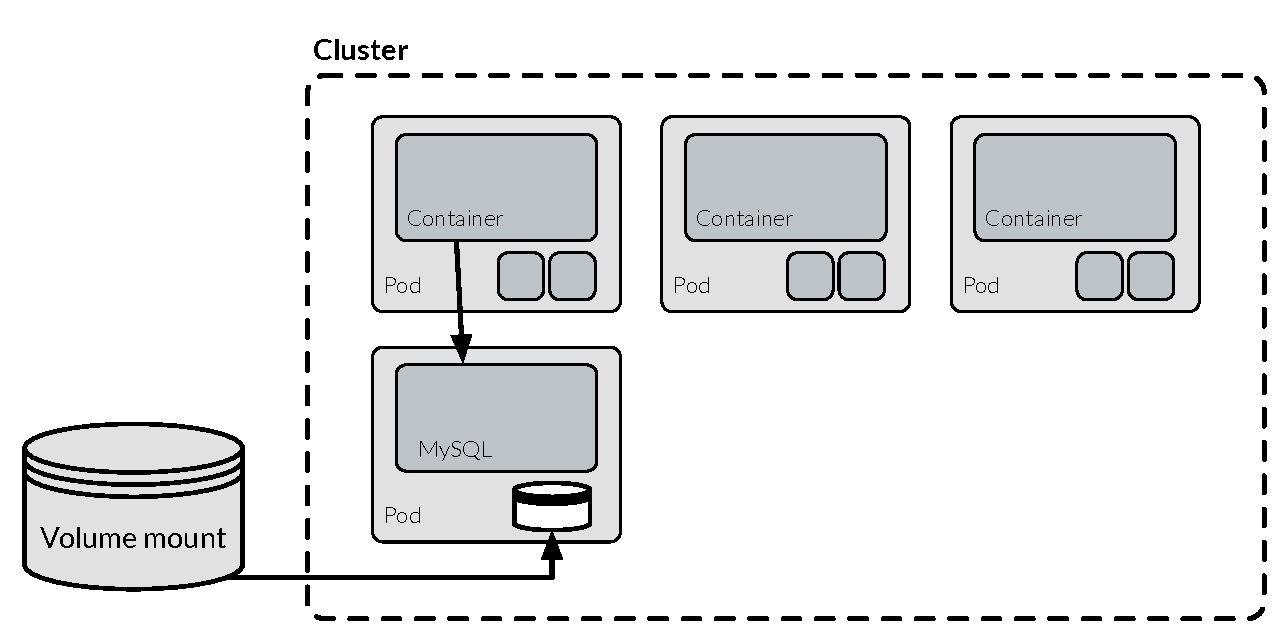
\includegraphics[width=12cm]{figures/appendix/database_adapt_cluster}
    \caption{Database Adapting to Cluster}
    \label{fig:db_adapt_cluster}
\end{figure}

\newpage
\subsection*{Cluster Native}
Databases such as Cassandra and Riak are designed to run in a distributed environment which is more cluster native approach. Availability, scalability, and fault tolerance are some of the benefits they provide. As described in Chapter~\ref{chap_fundamentals_resilient_cloud}, a trade-off between consistency and availability can be made e.g. in Cassandra depending. Sharding and replicating databases are factors used to achieve these benefits.

\begin{figure}
    \centering
    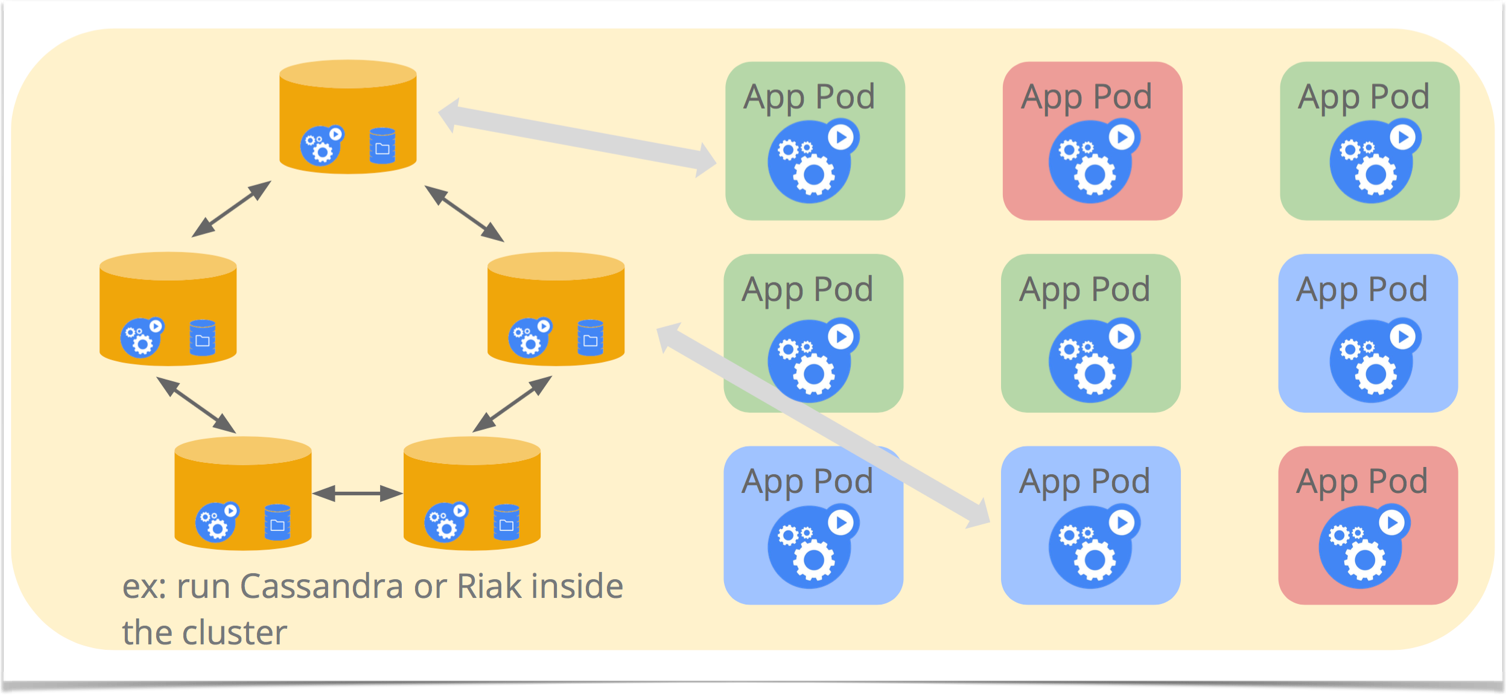
\includegraphics[width=\textwidth]{figures/appendix/database_cluster_native}
    \caption{Database Cluster Native}
    \label{fig:db_cluster_native}
\end{figure}

